\section{Auswertung}
\subsection{Vorgehen und genutzte Programme}
Zur Automatisierung der Auswertung wird wie folgt vorgegangen:
\begin{enumerate}
  \item Die Filme werden auf einem Scanner digitalisiert.
  Der Film der Salzprobe muss dabei während des scannens von oben beleuchtet werden,
  da der Film durch die längere Messdauer und Streulicht sehr stark belichtet
  wurde.
  \item Die gescannten Bilder werden digital nachbearbeitet, sodass die
  Beugungskreise besser hervortreten.
  \item Zwischen den Stanzungen der Filme werden die Grauwerte in einem schmalen,
  mittigen Streifen ausgelesen.
  Dazu wird das Programm ImageJ\cite{Schneider2012} genutzt.
  \item Die Grauwerte werden in einem Python\cite{python}-script
  durch Pandas\cite{mckinney-proc-scipy-2010} eingelesen.
  Der Grauwert wird invertiert und der Untergrund manuell auf ein
  einheitliches Niveau zu heben.
  \item Durch die Funktion \texttt{find\_peaks} der SciPy\cite{scipy}-Bibliothek
  \texttt{signal} werden die Peaks und damit die Beugungskreise detektiert.
  Die Abstände zum Mittelpunkt der Stanzung in Millimeter entsprechen dabei
  dem Winkel $\phi$ in Grad.
  \item Es werden helle und dunkle Peaks getrennt und die Analyse nur mit den dunklen
  fortgesetzt.
  Peaks, die durch eine K$_{\alpha_{1}}$- und eine K$_{\alpha_{2}}$-Linie
  entstanden sind, aber zu einem Tupel Millerindizes gehören, werde gemittelt.
  \item Für jeden Peak werden durch die Bragggleichung Netzebenenabstände
  berechnet. Anschließend werden die möglichen Millerindizes für ein bcc\footnote{$h+k+l$ gerade}-
  und ein fcc\footnote{$h, k, l$ Alle gerade oder ungerade}-Gitter
  aufsteigend nach $n=\sqrt{h^{2}+k^{2}+l^{2}}$ sortiert zugeordnet.
  \item Durch die SciPy-optimize Funktion \texttt{curve\_fit} wird ein linearer
  Fit durch die Gitterkonstanten beider Gittertypen in Abhängigkeit
  des $\cos{(\phi)}^{2}$ gelegt und der optimale Wert für die Gitterkonstante
  durch den y-Achsenabschnitt bestimmt.
\end{enumerate}

\subsection{Metallprobe}
Der Ausschnitt zwischen den Stanzungen des Films ist in \autoref{Abb:Metall}
zu sehen, die ausgelesenen Reflexe mit den zugeordneten Millerindizes für die
Hypothesen einer bcc- und einer fcc-Gitterstruktur finden sich mit den entsprechend
berechneten Gitterkonstanten in \autoref{Tab:Metall}.
Zusätzlich sind in \autoref{Abb:Metall_Peaks} die ausgelesenen Peaks eingezeichnet.
Eine Ausgleichsrechnung mit einer linearen Funktion für beide Gittertypen ist in
\autoref{Abb:Metall_a} gezeigt. Die bestimmte Steigung $m$ und der y-Achsenabschnitt $n$
finden sich in Tabelle \autoref{Tab:Metall_Regression}.
Es zeigt sich, dass die bcc-Hypothese stärke Schwankungen aufweist, was
sich auf einen größeren Fehler in der Ausgleichsrechnung niederschlägt.
Es liegt daher nahe, die bcc Hypothese als fehlerhaft anzusehen und ein fcc-Gitter
mit Gitterkonstante $a=\SI{342(13)}{\pico\metre}$ anzunehmen.


\begin{figure}
  \centering
  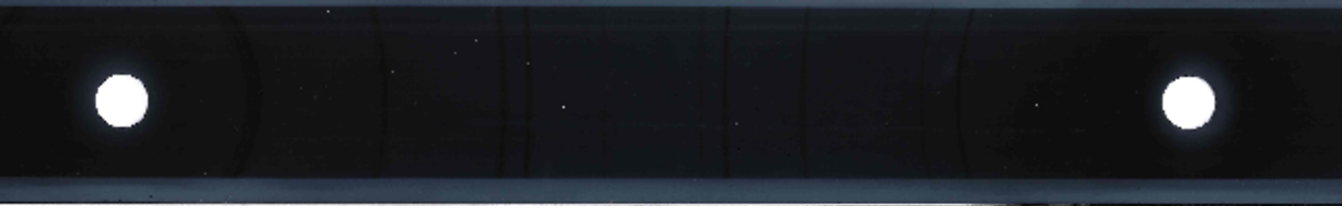
\includegraphics[scale=0.5]{content/pics/Metall_film.pdf}
  \caption{Filmaufnahme der Metallprobe. Der Winkel \SI{0}{\degree} liegt in der
  rechten, der Winkel \SI{180}{\degree} in der linken Stanzung}
  \label{Abb:Metall}
\end{figure}

\begin{table}[H]
  \centering
  \caption{Beugungsreflexe an der Metallprobe und zugeordnete Millerindizes
  und Gitterkonstanten für bcc und fcc-Gitter.}
  \label{Tab:Metall}
  \begin{tabular}{c || c c c c c|c c c c c}
    \toprule
    Winkel / ° &
    $n_{\text{bcc}}^{2}$ &
    $h_{\text{bcc}}$ &
    $k_{\text{bcc}}$ &
    $l_{\text{bcc}}$ &
    $a_{\text{bcc}}$ / pm &
    $n_{\text{fcc}}$ &
    $h_{\text{fcc}}$ &
    $k_{\text{fcc}}$ &
    $l_{\text{fcc}}$ &
    $a_{\text{fcc}}$ / pm\\
    \midrule
    40.35 & 2 & 1 & 1 & 0 & 315.92 & 3 & 1 & 1 & 1 & 386.92 \\
46.32 & 4 & 2 & 0 & 0 & 391.83 & 4 & 2 & 0 & 0 & 391.83 \\
65.61 & 6 & 2 & 1 & 1 & 348.32 & 8 & 2 & 2 & 0 & 402.21 \\
79.65 & 8 & 2 & 2 & 0 & 340.27 & 11 & 3 & 1 & 1 & 399.00 \\
112.63 & 10 & 3 & 1 & 0 & 292.80 & 12 & 2 & 2 & 2 & 320.75 \\
116.84 & 12 & 2 & 2 & 2 & 313.29 & 16 & 4 & 0 & 0 & 361.75 \\
136.84 & 14 & 3 & 2 & 1 & 310.01 & 19 & 3 & 3 & 1 & 361.15 \\
158.60 & 16 & 4 & 0 & 0 & 313.64 & 20 & 4 & 2 & 0 & 350.66 \\

    \bottomrule
  \end{tabular}
\end{table}

\begin{figure}[h!]
  \centering
  \subcaptionbox{Zur Position in \autoref{Abb:Metall} korrespondierende
  Peaks. \label{Abb:Metall_Peaks}}[0.45\textwidth]{
  \centering
  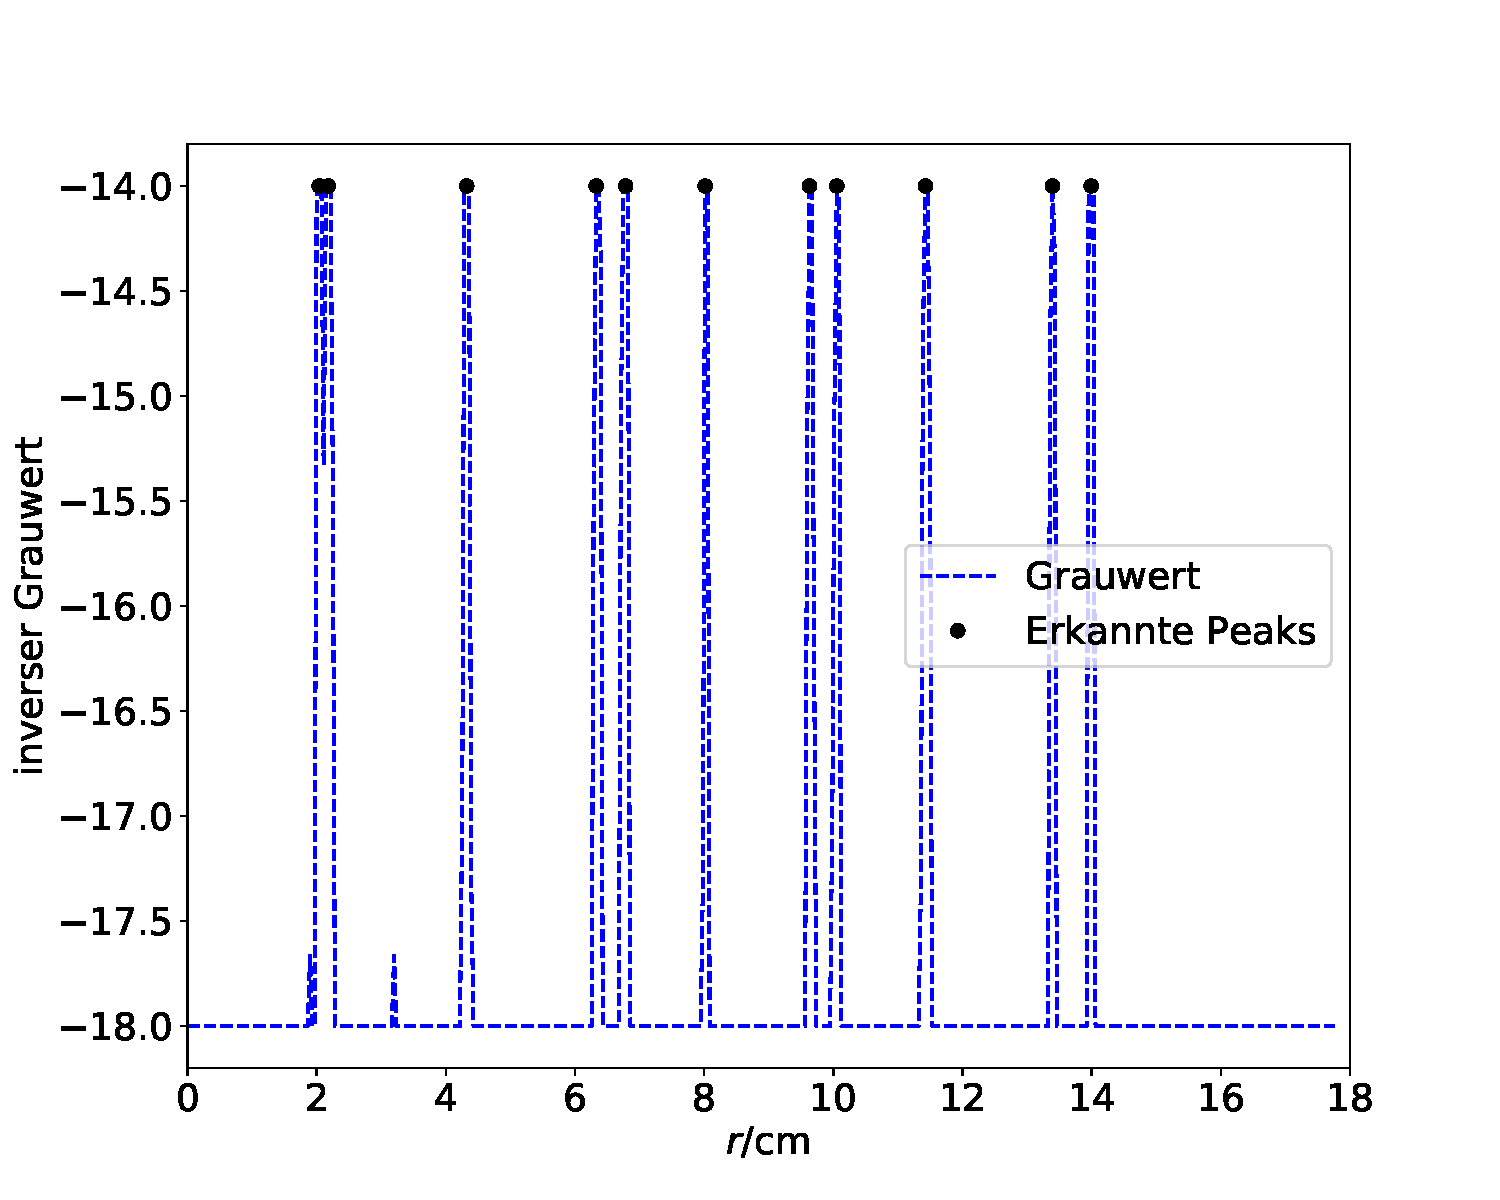
\includegraphics[width=0.45\textwidth]{Auswertung/Grafiken/Metall_Peaks.pdf}
  }
  \subcaptionbox{Gitterkonstante mit Ausgleichsrechnung. Die Position der Peaks wurde
  dafür invertiert. \label{Abb:Metall_a}}[0.45\textwidth]{
  \centering
  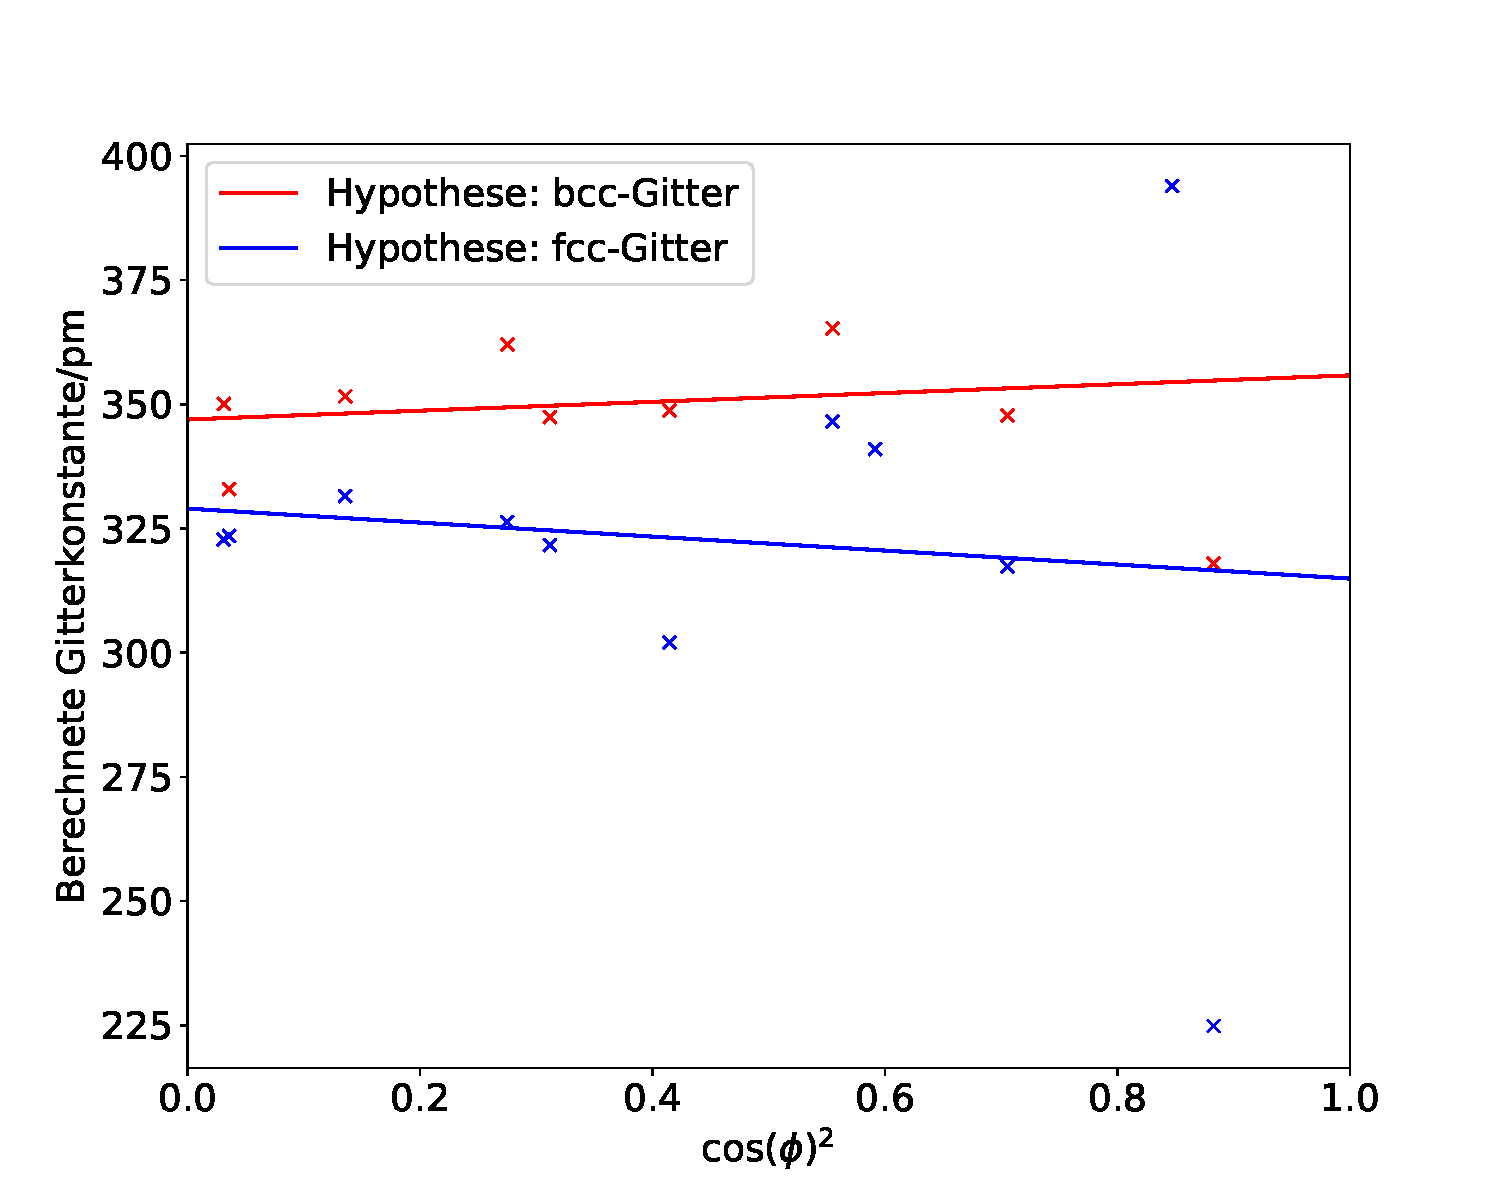
\includegraphics[width=0.45\textwidth]{Auswertung/Grafiken/Metall_Ausgleichsrechnung.pdf}
  }\\
  \label{Abb:Metall_Plots}
  \caption{Grafiken für die Metallprobe.}
\end{figure}

\begin{table}[H]
  \centering
  \caption{Parameter der Ausgleichsrechnung für die Metallprobe.}
  \label{Tab:Metall_Regression}
  \begin{tabular}{c | c c }
    \toprule
    Gittertyp &
    $m$ / $\frac{\mathrm{pm}}{1}$ &
    $n$ / pm \\
    \midrule
    bcc & \num{60(30)} & \num{300(17)} \\
    fcc & \num{63(24)} & \num{342(13)} \\
    \bottomrule
  \end{tabular}
\end{table}

\subsection{Salzprobe}
Der Ausschnitt zwischen den Stanzungen des Films ist in \autoref{Abb:Salz}
zu sehen, die ausgelesenen Reflexe mit den zugeordneten Millerindizes für die
Hypothesen einer bcc- und einer fcc-Gitterstruktur finden sich mit den entsprechend
berechneten Gitterkonstanten in \autoref{Tab:Salz}.
Zusätzlich sind in \autoref{Abb:Salz_Peaks} die ausgelesenen Peaks eingezeichnet.
Aufgrund der starken Belichtung des Films und der zusätzlichen Verunreinigung durch Streulicht
war es nicht möglich, helle und dunkle Reflexe zu trennen.
Wider ist eine Ausgleichsrechnung mit einer linearen Funktion für beide Gittertypen in
\autoref{Abb:Salz_a} gezeigt. Die bestimmte Steigung $m$ und der y-Achsenabschnitt $n$
finden sich in Tabelle \autoref{Tab:Salz_Regression}.
Es zeigt sich, dass die fcc-Hypothese weitaus stärke Schwankungen aufweist, was
sich auf einen größeren Fehler in der Ausgleichsrechnung niederschlägt.
Es liegt daher nahe, die fcc Hypothese als fehlerhaft anzusehen und ein bcc-Gitter
mit Gitterkonstante $a=\SI{369(6)}{\pico\metre}$ anzunehmen.

\begin{figure}
  \centering
  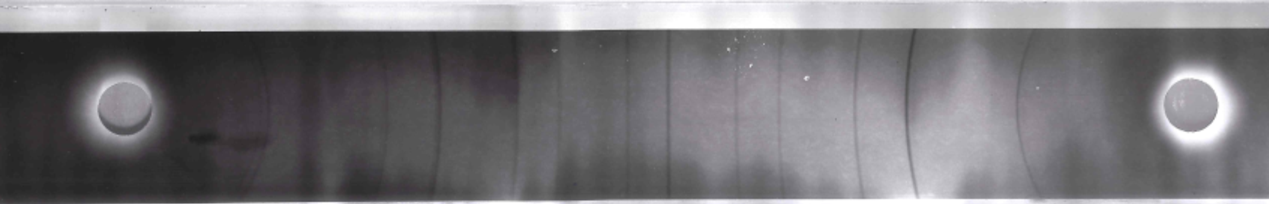
\includegraphics[scale=0.5]{content/pics/Salz_film.pdf}
  \caption{Filmaufnahme der Salzprobe. Der Winkel \SI{0}{\degree} liegt in der
  rechten, der Winkel \SI{180}{\degree} in der linken Stanzung. Es ist ein
  deutlicher Verlauf von dunkel (links) nach hell (rechts) zu erkennen, der durch
  einfallendes Streulicht verursacht wurde.}
  \label{Abb:Salz}
\end{figure}

\begin{table}[H]
  \centering
  \caption{Beugungsreflexe an der Salzprobe und zugeordnete Millerindizes und Gitterkonstanten
  für bcc und fcc-Gitter.}
  \label{Tab:Salz}
  \begin{tabular}{c || c c c c c|c c c c c}
    \toprule
    Winkel / ° &
    $n_{\text{bcc}}^{2}$ &
    $h_{\text{bcc}}$ &
    $k_{\text{bcc}}$ &
    $l_{\text{bcc}}$ &
    $a_{\text{bcc}}$ / pm &
    $n_{\text{fcc}}$ &
    $h_{\text{fcc}}$ &
    $k_{\text{fcc}}$ &
    $l_{\text{fcc}}$ &
    $a_{\text{fcc}}$ / pm\\
    \midrule
    30.82 & 3 & 1 & 1 & 1 & 502.25 & 1 & 1 & 0 & 0 & 289.98 \\
49.38 & 4 & 2 & 0 & 0 & 368.92 & 2 & 1 & 1 & 0 & 260.86 \\
58.13 & 8 & 2 & 2 & 0 & 448.56 & 3 & 1 & 1 & 1 & 274.69 \\
70.74 & 11 & 3 & 1 & 1 & 441.45 & 4 & 2 & 0 & 0 & 266.21 \\
78.09 & 12 & 2 & 2 & 2 & 423.68 & 5 & 2 & 1 & 0 & 273.48 \\
89.30 & 16 & 4 & 0 & 0 & 438.53 & 6 & 2 & 1 & 1 & 268.54 \\
96.30 & 19 & 3 & 3 & 1 & 450.84 & 8 & 2 & 2 & 0 & 292.54 \\
107.86 & 20 & 4 & 2 & 0 & 426.28 & 9 & 2 & 2 & 1 & 285.96 \\
114.51 & 24 & 4 & 2 & 2 & 448.75 & 9 & 3 & 0 & 0 & 274.81 \\
127.82 & 27 & 5 & 1 & 1 & 445.77 & 10 & 3 & 1 & 0 & 271.28 \\
136.58 & 27 & 3 & 3 & 3 & 430.92 & 11 & 3 & 1 & 1 & 275.05 \\
157.24 & 32 & 4 & 4 & 0 & 444.58 & 12 & 2 & 2 & 2 & 272.25 \\

    \bottomrule
  \end{tabular}
\end{table}

\begin{figure}[h!]
  \centering
  \subcaptionbox{Zur Position in \autoref{Abb:Salz} korrespondierende
  Peaks. \label{Abb:Salz_Peaks}}[0.45\textwidth]{
  \centering
  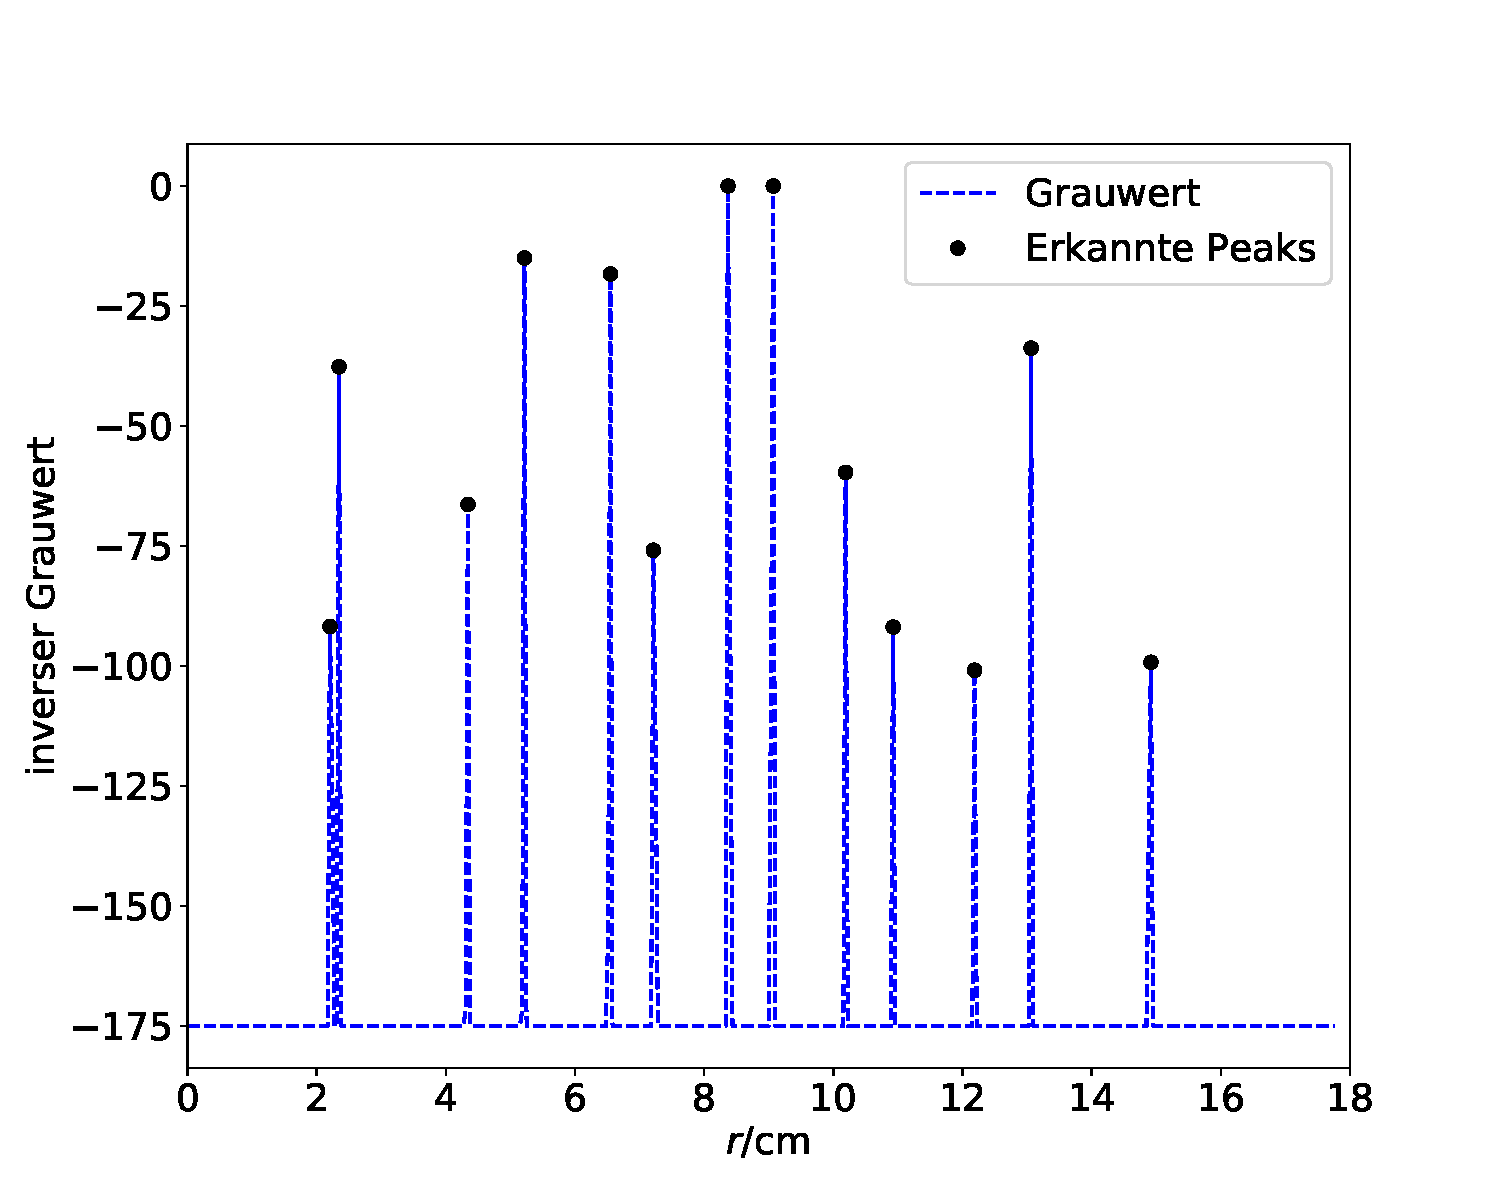
\includegraphics[width=0.45\textwidth]{Auswertung/Grafiken/Salt_Peaks.pdf}
  }
  \subcaptionbox{Gitterkonstante mit Ausgleichsrechnung. ie Position der Peaks wurde
  dafür invertiert. \label{Abb:Salz_a}}[0.45\textwidth]{
  \centering
  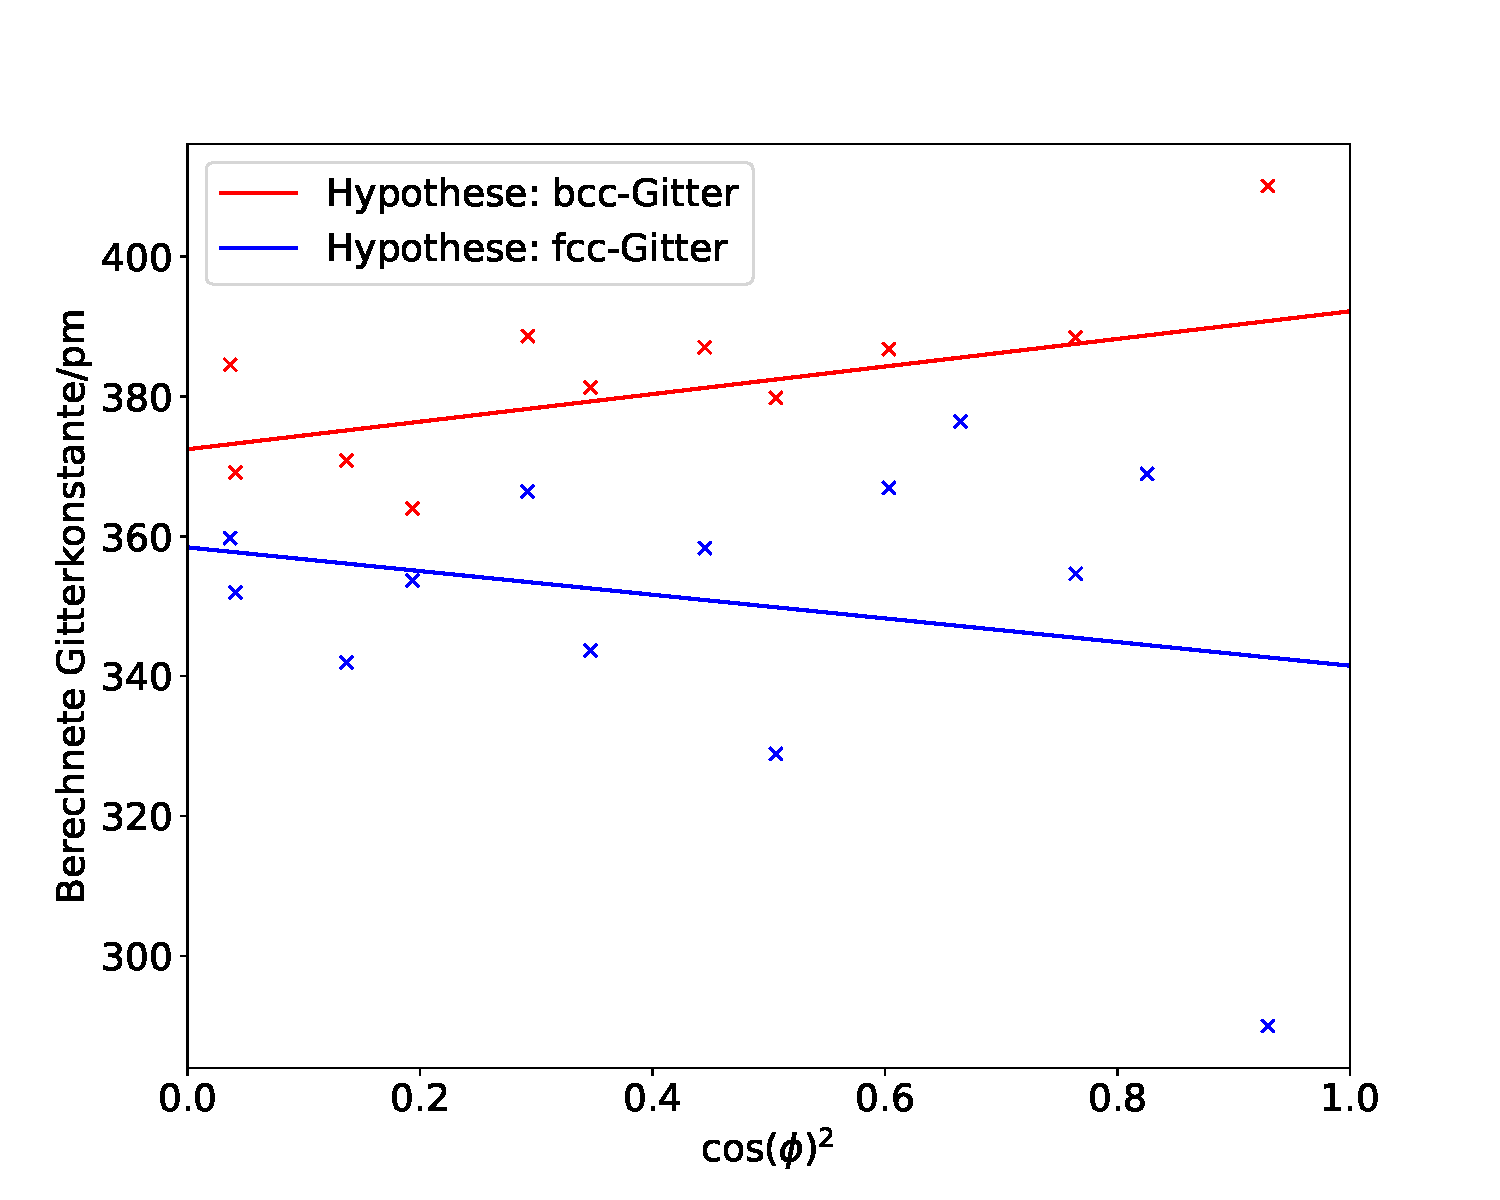
\includegraphics[width=0.45\textwidth]{Auswertung/Grafiken/Salt_Ausgleichsrechnung.pdf}
  }\\
  \label{Abb:Salz_Plots}
  \caption{Grafiken für die Salzprobe.}
\end{figure}

\begin{table}[H]
  \centering
  \caption{Parameter der Ausgleichsrechnung für die Salzprobe.}
  \label{Tab:Salz_Regression}
  \begin{tabular}{c | c c }
    \toprule
    Gittertyp &
    $m$ / $\frac{\mathrm{pm}}{1}$ &
    $n$ / pm \\
    \midrule
    bcc & \num{26(11)} & \num{370(6)} \\
    fcc & \num{0(40)} & \num{437(18)} \\
    \bottomrule
  \end{tabular}
\end{table}

\section{Diskusion}
Die Metallprobe zeigt gut auszuwertende Ergebnisse. Aufgrund der guten Abschirmung
konnten schwache, helle Reflexe gut erkannt werden, die in der weiteren Auswertung
nicht weiter berücksichtigt wurden. Mit einer Gitterkonstante von $\SI{342(13)}{\pico\metre}$
bewegt sich das Analyseergebnis in einem für Metalle typischen Bereich.\\
Im Gegensatz dazu liegt die bestimmte Gitterkonstante der salinen Probe mit
$a=\SI{369(6)}{\pico\metre}$ bei einem für Salze ungewöhnlich niedrigen Wert.
Zwar gibt es Salze mit einer solch niedrigen Gitterkonstante, es kann aber nicht
ausgeschlossen werden, dass hier Fehlinterpretationen auftreten. Insbesondere
die starke Kontamination durch Streulicht kann dazu führen, dass in Wahrheit schwache,
helle Reflexe in der Analyse genutzt werden, die eigentlich ignoriert werden müssten.
Dafür spricht, dass die in \autoref{Abb:Salz_a} bei hohen $\cos{(\phi)}^{2}$-Werten
zu sehenden Ausreißer in den durch Streulicht stark verschmutzten Bereich des
Films fallen. Um systematische Fehler auszuschließen wäre hier eine wiederholte
Vermessung der Probe angebracht.
